\chapter{Calibration Procedures}

This manual is meant to walk the user through calibrating the situational awareness system of the CS Saucer. It encompasses the camera calibration and then the lidar and camera calibration procedures. 

\section{Camera calibration}

First, make sure that the camera is correctly mounted, and that the ribbon cable is connected to the Raspberry Pi. For this calibration, you will need a checkerboard pattern. You can find some in the MC Lab, or print out your own on an A3 paper. It is recommended that you laminate the checkerboard so you can use it multiple times. The pattern used in this thesis was 9x7 squares with the length of 40 mm. The exact number and size is arbitrary as long as it is specified to the software. Place the Saucer somewhere high enough that you can move quite freely in the camera frame. 

SSH on to the Raspberry pi via your operator computer, and run the camera driver as outlined in \cref{sec:camera-driver}. Then in a separate terminal window on the operator computer (not the RPi!) run the following comand:

\begin{lstlisting}[language=bash]
$ rosrun camera_calibration cameracalibrator.py --size 8x6 --square 0.40 image:=/cv_camera/raw_image camera:=/cv_camera
\end{lstlisting}

Here --size is the argument for number of inner corners in the pattern and --square the length of the sides. If the node is successfully activated, you will be met with the following window: 

\begin{figure}[H]
    \centering
    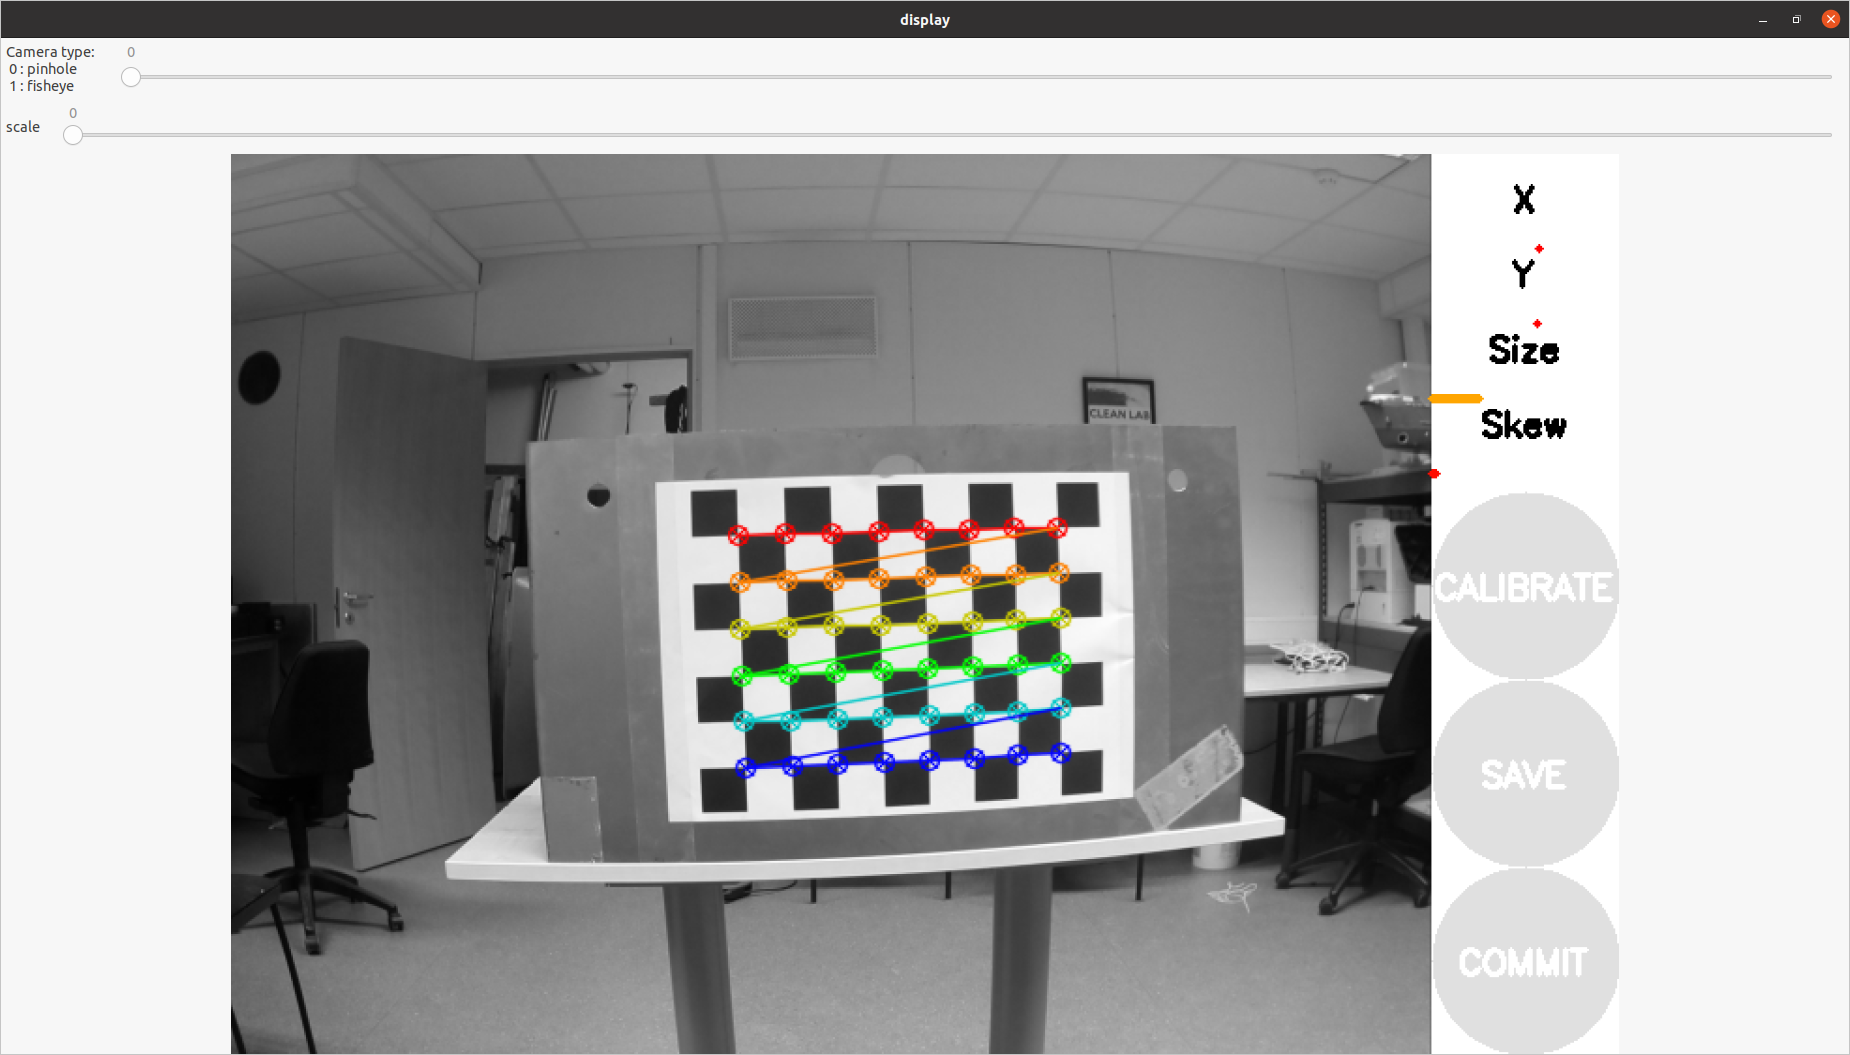
\includegraphics[width=\textwidth]{Images/camera-calibration.png}
    \caption{Calibration window}
    \label{fig:calibration-window}
\end{figure}

Move the checkerboard around in different orientations, at different distances in the camera frame. The program will grab data-samples as you go. When the bars on the right of \cref{fig:calibration-window} are full enough, the calibrate button will turn a darker shade of grey. This means that enough data has been collected to produce a calibration. You can keep going to produce a more accurate calibration. When you are finished, simply press the cailbrate button and the procedure will start. After it is over, the intrinsic parameters will be printed to the terminal window. To save these, press commit. This will make sure that the camera driver on the raspberry pi, always launches with these intrinsic parameters. You can also save the parameters to a file using the 'Save' button. Now you can exit the window. 

\section{Camera-Lidar calibration}

The software for the lidar-camera calibration is based on \cite{calibration-repo}. However, some changes have been made, so it is recommended that you use the files provided electronically with the thesis. Copy the calibration workspace over to your operator computer, and build it. Make sure you clean the files in the directory \textit{data}. In the directory calle \textit{config}, edit the config.yaml file to contain the intrinsic camera  parameters you obtained from the camera calibration.

Next you should identify the geometry you wish to use as your anchor points, and measure the height up to the lidar from the floor. Then, mark that height with tape on the corners inside the cameras point of view. 

Then you can SSH onto the RPi and start the lidar and camera according to \cref{sec:lidar-driver} and \cref{sec:camera-driver}. On the operator computer, in the calibration workspace, run the command 

\begin{lstlisting}[language=bash]
$ roslaunch camera_2d_lidar_calibration collect_camera_calibration_data.launch
\end{lstlisting}

This will print you camera parameters in the terminal and activate the program RViz, as seen in \cref{fig:yup}

\begin{figure}[H]
    \centering
    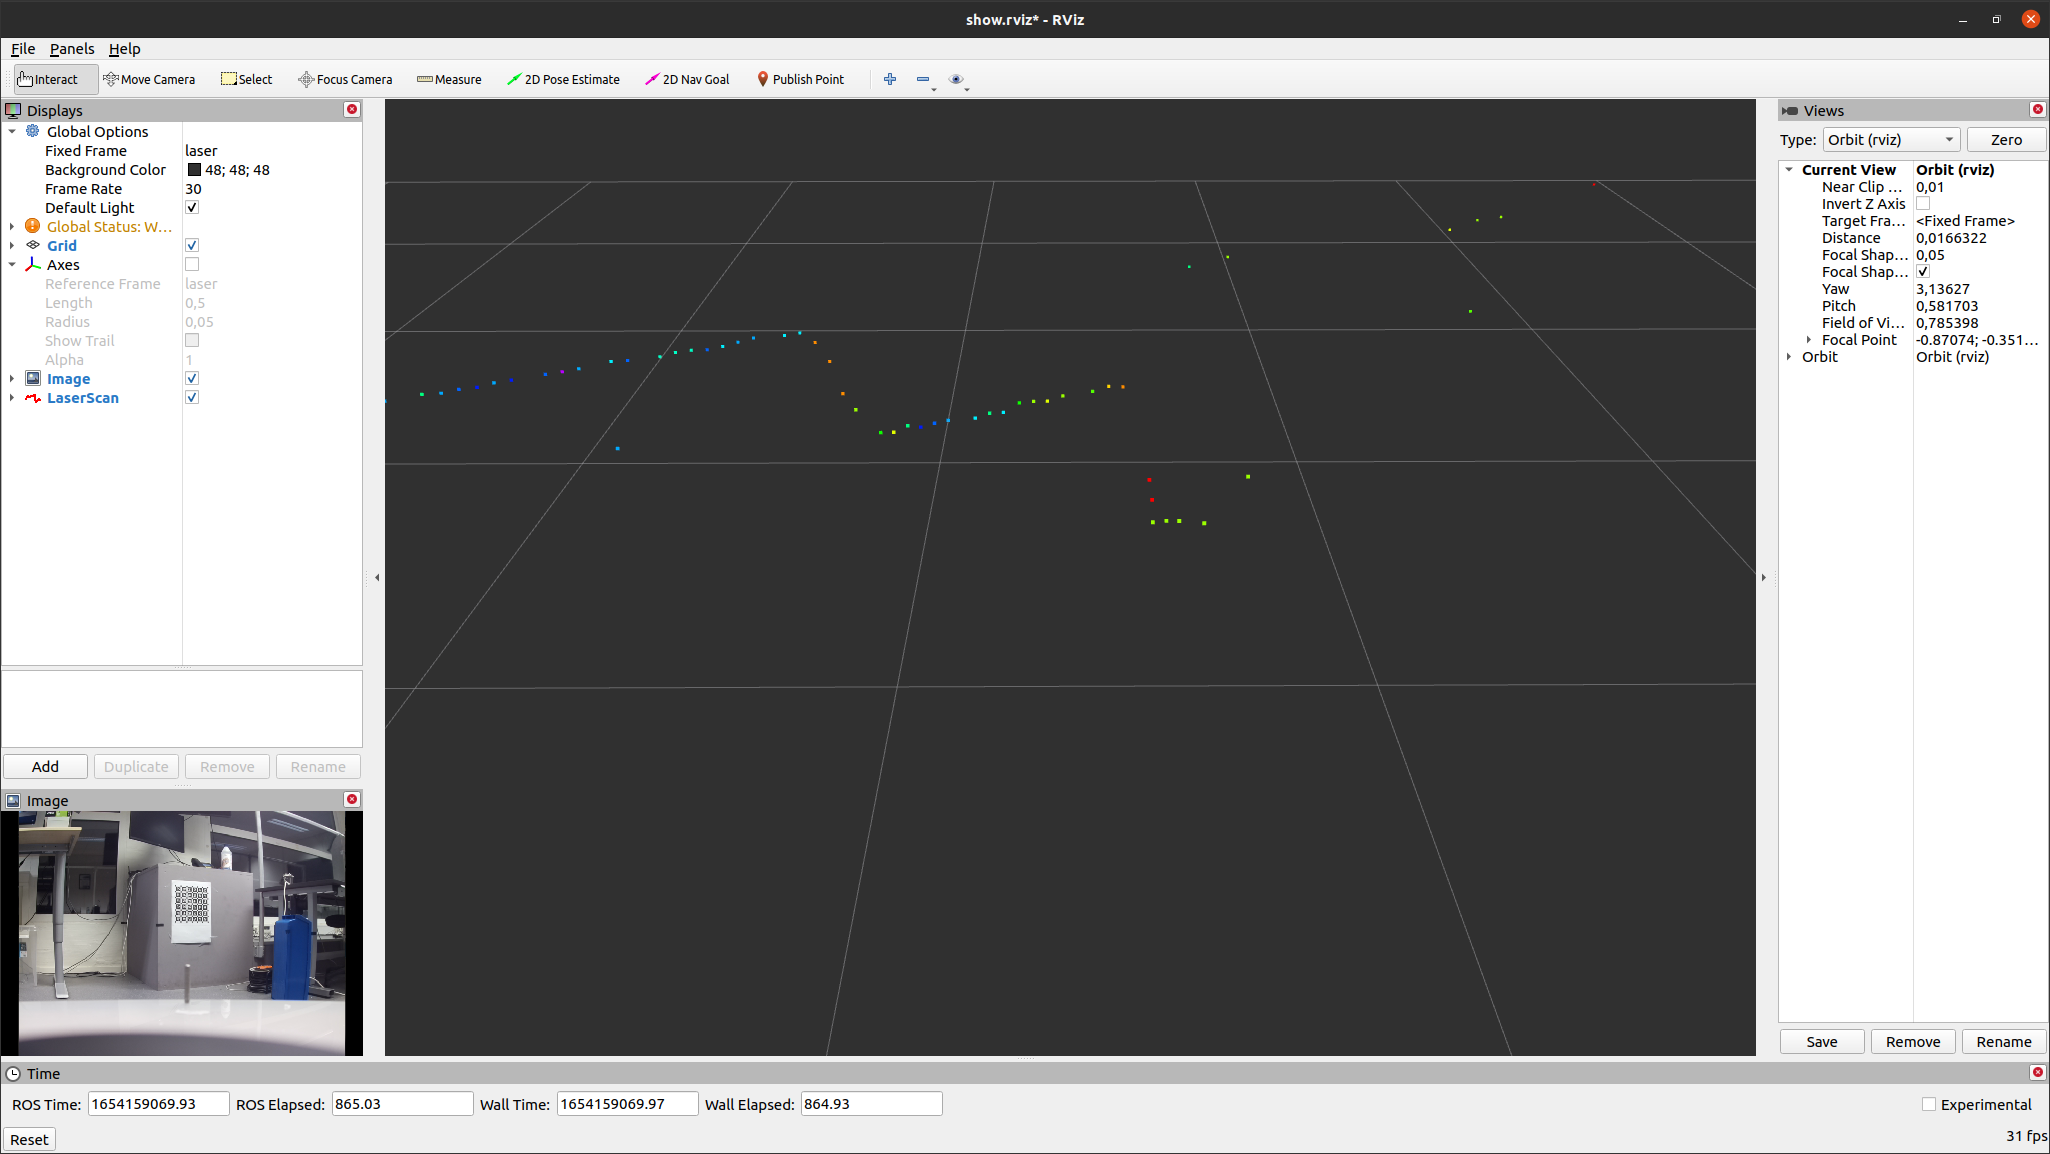
\includegraphics[width=\textwidth]{Images/actual-laz-cal.png}
    \caption{RViz window for calibration}
    \label{fig:yup}
\end{figure}

Then using the \textbf{2D Nav Goal} tool from the top bar, pick a point from the laser point cloud that corresponds to a corner. This will prompt the following window in \cref{fig:pixel-value}


\begin{figure}[H]
    \centering
    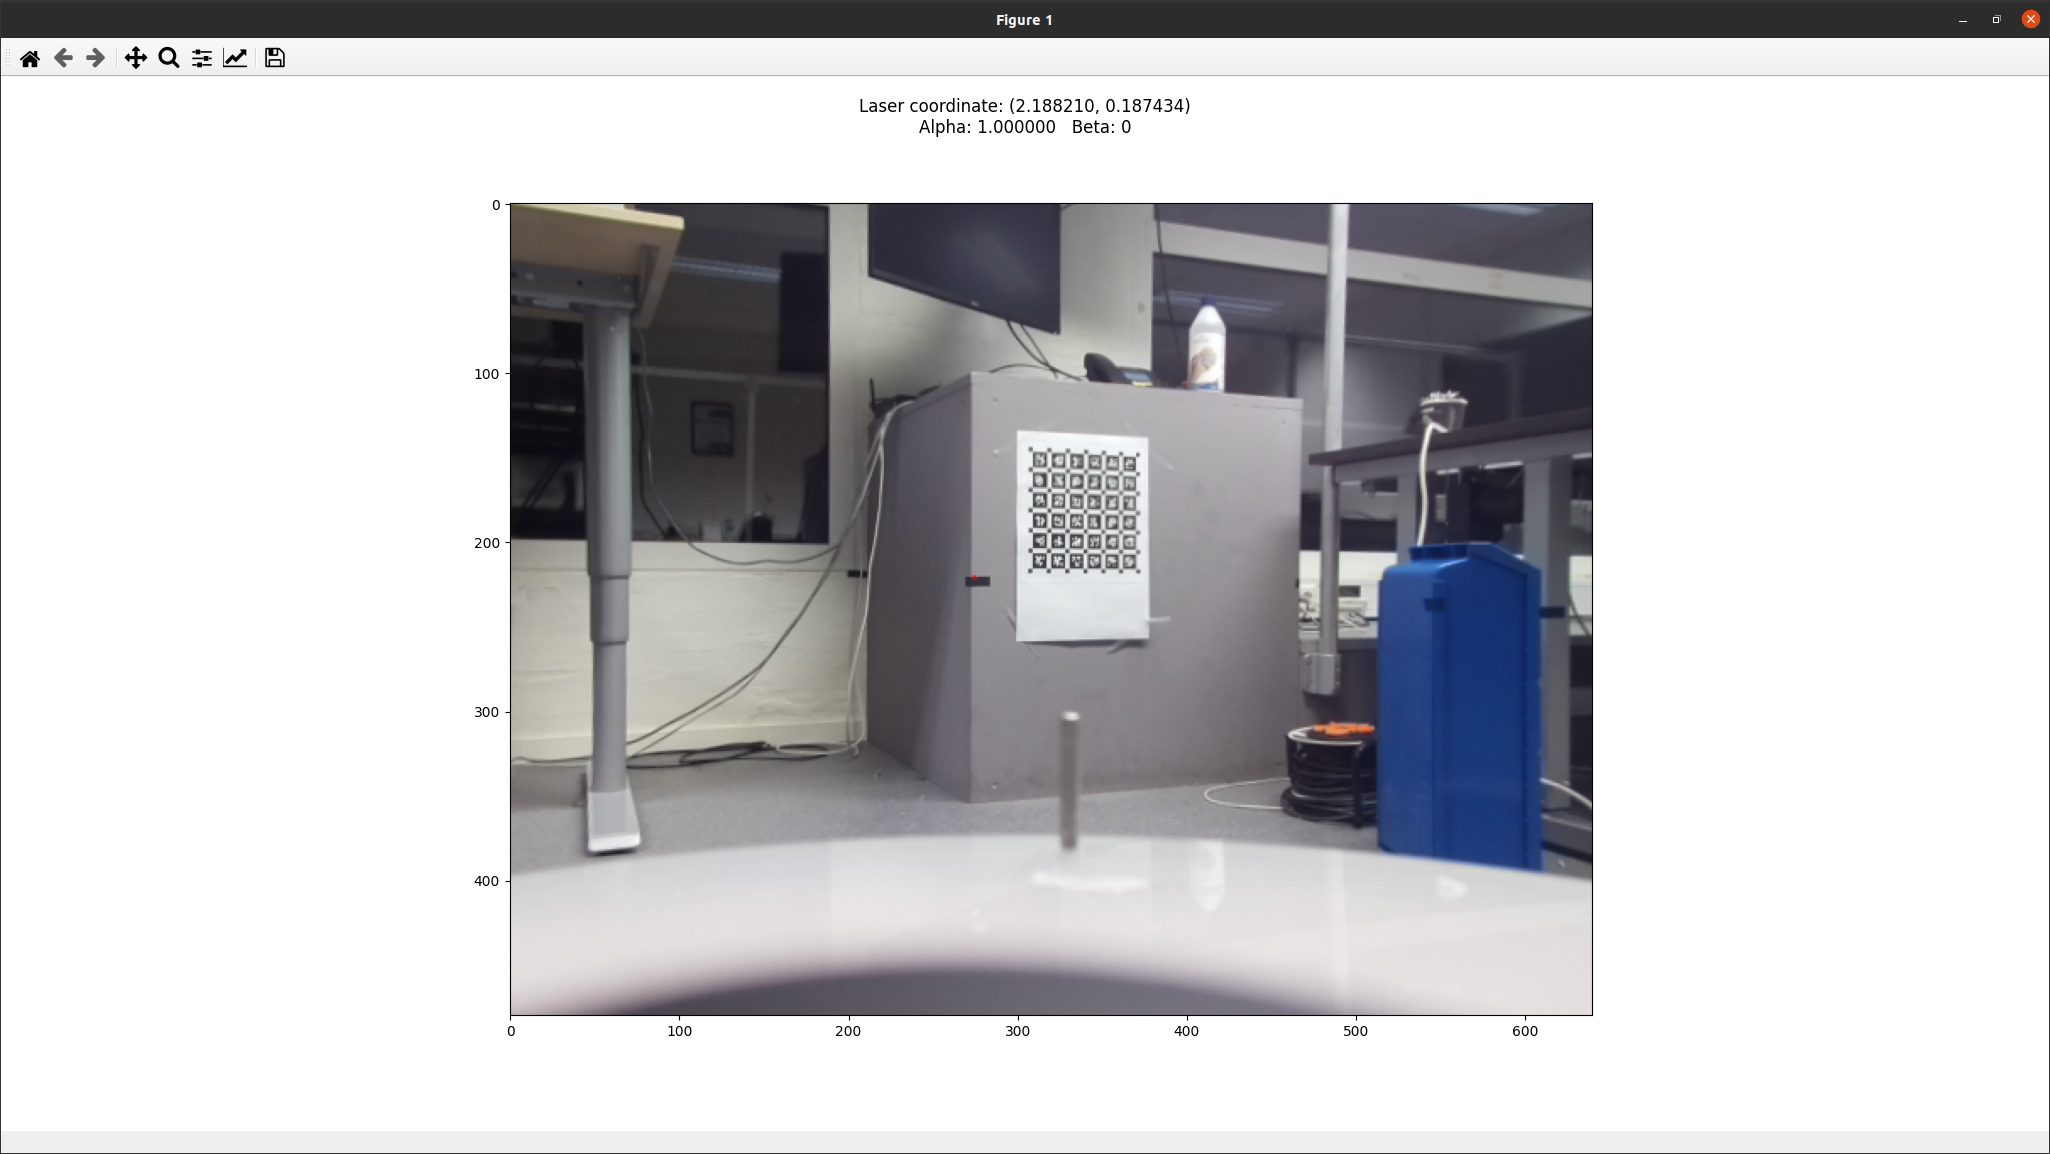
\includegraphics[width=\textwidth]{Images/choose-point.png}
    \caption{Choosing corresponding pixel value}
    \label{fig:pixel-value}
\end{figure}

Mark the area in the image that corresponds to the lidar point you chose. This is not an exact science, but try to be as accurate as you can. When satisfied with the point placement, press space and the window will close and the point be saved. Repeat the process several times for all the corners until you get enough data points. 10-20 should suffice, try to reduce the RMSE as much as possible. After you have enough data, close RViz and in the terminal run the second command

\begin{lstlisting}[language=bash]
$ roslaunch camera_2d_lidar_calibration calibration.launch
\end{lstlisting}

This will run the camera and lidar calibration procedure and spit out the rigid body transformation along with the root mean square error. You can check the translation with hand-measurements, if they are in the same ballpark the calibration is ok. You can now try to reproject the laser point onto the live image. This is done by running 

\begin{lstlisting}[language=bash]
$ roslaunch camera_2d_lidar_calibration reprojection.launch
\end{lstlisting}

Here you can see how the lidar points line up with the tape. 